\setcounter{chapter}{ 10 }
\chapter{\textbf{SAC-09, Interlude} }



\subChapterTitle{``Didn't Even Have Nails in Them''} 

\deets{Suko}{November 28th, 2012}



Jaya's Worst Week Ever (again).  



As always, p\hl{lease fill in the gaps and correct errors}\footnote{\textbf{Suko T }Thanks for all the edits/additions Rebecca and Ion!  I love having these be a collaborative documents and getting Jonah and Jaya's perspective too.  Re-reading these later is going to be awesome.  :) \textsubscript{11/30/12 2:46pm}}.  Also you should always feel free to add/correct the perspective of your character.

\jumpHeadline{ Capability purchases } 

Jaya: \textit{Stash: 1 → 2} and \textit{Senior Constable: 1 → 2}

Hayley: Reduce Flaw: Follower: \textit{1{[}2{]} → 0{[}3{]}}, Reduce Flaw: Fear: \textit{2{[}0{]} → 1{[}1{]}} (via Capability expenditure)

\jumpHeadline{ SAC-09 } 


\sceneHeadline{Jaya's New Assignment }

Jaya is called in to speak with Agent Morgan in Ops.  Agent Rook and Tech Larissa are there.  Rook is sitting near the tanks, across the table from Morgan.



Jaya asks if she can go on Shore Leave now.  Morgan says that she has a personnel issue that she was hoping to get Jaya's help with.  ``We have a limited headcount here but we are still required to give our assistance in police authority issues.  We have to send someone, who would you suggest?''  \hl{Jaya's ego is clearly stroked at being asked this}\footnote{\textbf{q.google }It seemed pretty clear to me that Morgan was very carefully and deliberately doing the stroking.  She never said ``No, Senior Constable, you're going'' and yet I interpreted that as what she wanted.  I'm not sure if OOG knowledge colored that though. \textsubscript{11/30/12 1:30pm}}.



Upon learning the job is potentially dangerous Jaya immediately volunteers Oliver, but Morgan asks if he is truly recovered enough to go on the mission.  Jaya then tries to suggest Lackovich (``to give her more experience'') but then finds out that there is money involved (hazard pay) and quickly volunteers herself.



Turns out the job is in the Annex, so after she has completed it, she can go on her Shore Leave if she wishes.  Jaya takes the deal.  Agent Morgan instructs her to get a standard uniform and baton.  She doesn't even have time to go back to her bunk- she's leaving right away.



Agent Tiburon Rook drives the train to Gateway Station and gives Jaya a note with a name and an order number on it. ``Go see him, he should be in his office.  He's in charge, you're our detachment to him.''  Jaya is at first put out that she won't be the senior officer in the area but settles down.



She tries to get Tiburon to give her some additional info or gossip on the situation, but Tiburon just stares at her impassively and she gives up.



Jaya saunters down the street, making sure to flash her badge and let everyone know a Senior TA officer is coming through.  She arrives at the building and there is a woman sitting outside with a book.  Jaya requests to see Chief Constable Anastasios, and after a short wait, is admitted into his office.  



There are two other Senior constables and one Agent.  Jaya likes Chief Constable Anastasios right away after seeing the tattoos peeking above his collar and seeing the facial scars of someone who's been in a lot of fights.  The Agent has a chiseled, more polished look and the two Senior Constables are fairly young, younger than Jaya.



After confirming that she is the detachment from Agent Morgan (``She told me she was sending one of her best.  Are you?''), the Chief quizzes her on her experience: if she knows how to use the baton she carries and if she has commanded before.  Jaya naturally says yes and brags a little.



Jaya learns that her assignment is to work the water station Gamma.  She will inspect the water shipments daily, 2 hours after sunrise and 2 hours before sunset.  Then she will dispense the water according to water credits.  If the shipment is delayed, she is to send a runner immediately.  She will be doing this for a week.



Jaya asks about the danger, and is told that there has been water rationing and this has caused some discontent.  She will have three junior constables, none of them well trained.  She'd have to train them.  When asked if that will be a problem, Jaya proudly boasts that she has already been working with a constable trainee and been making great progress, so this should be no problem.



Jaya is given a new badge (green with seven points and irregularly sized sides).



``Oh one more thing.  Feel free to make examples,''  says Chief Constable Anastasios.  Jaya smiles, salutes and leaves.



The post is hellish.  Jaya gets very little sleep, but there is also very little to do, so she's bored and exhausted.  The water costs have gone up about 30\% and people are annoyed.  Jaya is constantly thwarting break-ins and scuffles from disgruntled people.  One of her constables gets pretty hurt and has to return back to the main post, so Jaya ends up short handed and running double duty, making her even more exhausted.  Jaya beats two of the people so badly that they die (or come close to it).  After that demonstration of brutality, the people are much less aggressive but there is more grumbling.



At the end of the week, Jaya gets a note to return to the post and a note from Morgan giving her 3 days of Shore Leave.



\sceneHeadline{Shore Leave: Jaya }

Jaya goes home to play the game of ``whose life is harder'' with her sister.  Jaya walks into LA Ink unannounced and declares FML.



Padme is unimpressed.  ``Why does this always have to be about you?''  The shop is empty - no one can afford tattoos these days.  Micah is nowhere to be seen.  Jaya finds that not only is Simon \underline{ \textit{not } }coming home, the annoying Joseph has gone off to work to help feed the family.  Padme thinks she's expecting again too.



Padme accuses Jaya of never being there and just lazing around while the family is working hard and suffering.  Jaya is indignant and reminds Padme of all the checks she sends home- every paycheck.  Jaya details the horrors of her latest assignment, doing water rationing @ the 7th. Padme says that things are getting bad.  Just recently someone had come in and beat her up and implies/figures out it may have had something to do with Jaya's work. 



Attempting to prove she is helpful and cares for the family, Jaya extends the peace offering of a new tattoo design for Padme to use, based on the caduceus symbol.  Padme gives her shit for trying to act like she knows everything, while pocketing the design, and fires back that what would be really helpful is if Jaya could have a kid.  Jaya abruptly leaves.



After getting shitfaced at one of the local bars, Jaya drunkenly hunts down the guy who beat up her sister.  Her keen deductive skills being somewhat impaired, it's possible the fellow she found had nothing whatsoever to do with her sister's beating but Jaya finds it very satisfying to beat him to a pulp.  She spends the rest of her Shore Leave in an inebriated haze.



She nearly misses her pickup train and when she finally does make it to the train back to SAC-09, she is simultaneously drunk and hungover (and still exhausted from lack of sleep).  She looks horrible, as she hasn't done more than a token clean up from her fight and her hair is greasy and matted with dried blood and other unmentionable things.



\sceneHeadline{SAC-09: Jonah }

Jari comes to find Jonah and tells him that Dr. Gerhauser would like to see him.  Jonah looks up from the book he is studying and asks Jari, ``How does she remember all of this?''  Jari doesn't know but says, ``She's been doing it a long time.''



They head down to Medbay and Jonah chats up Jari, getting to know him a little better, asking what he does for fun around here.  Jari does play cards but he's not very good at it.  He also enjoys cooking, and he likes organizing, wry pointing out that this is a good thing, given that organizing is his job.



Dr. Gerhauser is waiting and asks how Jonah is doing.  

``A bit confused.  There are a lot of words in that book,'' Jonah replies.

``Are you sleeping okay?  Jari says that your appetite is alright, or at least within expected parameters.''

Dr. Gerhauser takes Jonah's blood pressure and a few other simple tests.  Jonah asks, ``How often do you use the information in that book?''

``Personally, not often.  Surgeons use it more often.  It is good to know so that if there is a problem, you can figure it out.''

``In my experience you don't have time to think about it, you have to fix what's trying to pour out, no matter what it's called.''

``Your people are relatively short lived and experience a lot of trauma.''

Jonah \hl{looks at her sharply}\footnote{\textbf{q.google }Dr. G knows, and Jonah knows that she knows.  It's a very unstated sort of knowing as a rule, but when Dr. G slips Jonah wants (needs) to find out why she slipped. \textsubscript{11/30/12 1:36pm}}, ``'Your people'?''

``Ah, from \hl{Gateway}\footnote{\textbf{Suko T }Where ``Jonah'' is from \textsubscript{11/30/12 12:21am}},'' says Dr. Gerhauser.

``Oh, so you mean like cops?'' inquires Jonah further.

``Yeah,'' says Dr. Gerhauser and then briskly changes the subject.  ``I understand you will be going in the Tank soon.''

``Who chooses that?''

``Your commanding officer said that you were ready.  I can take some baseline measurements now and prep you for the Tank, or we can do it after you return from Shore Leave.''

``What does it involve?'' asks Jonah.

Dr. Gerhauser shows him the cap with the leads coming out of it and says that she'll put it on his head and ask him some questions.  Jonah agrees to the baseline now but the prep will wait until after he returns from Shore Leave.  otherwise the delay may throw the schedule too far off.



Dr. Gerhauser puts the cap on him and starts asking questions.

``What is the most interesting thing in the book?''

``There is a lot more shape to things than I expected.  Usually when I see insides, they are a mess.''

``When was the first time you saw someone's insides?''

``During the Bucket Riots.''

``And you weren't a medic then?''

``Yes I was, but I hadn't been a medic for very long.''

``Tell me about your mother.''

``She's mostly tired.  I haven't seen her in a while.''

``How many grams in a liter?''

``1000,'' Jonah replies, but is not entirely confident in his answer.

``What do you think about your superior officer?''

``Which one?''

``Hmm, which one pops to mind first?''

``Rook.''``Really?''.  Dr. Gerhauser is surprised. ``Not the Senior Constable?''Jonah \hl{hesitates}\footnote{\textbf{q.google }Because he isn't sure if he should give the actual answer (he does) but can't come up with anything else. \textsubscript{11/30/12 1:39pm}}.  ``Because I don't know him very well.''

``Who is your best friend?''

``Tareq.  I worked with him before I was a constable.  He was a medic too.''

``What does yellow skin indicate?''

``Under the skin, or on the surface?'' asks Jonah

``Under.''

``Face or torso?''

``All over.''

``A liver problem, most likely,'' replies Jonah.

Dr. Gerhauser nods slightly before continuing.

``How many bones in the human body?''

``208, according to that book, although they were counting the very very tiny bones and the large bones each as one.''

``Are you sexually active?''

``No.''

``Do you have kids?''

``No.''

``When you were a child, what were you most afraid of?''

Jonah thinks about his answer for a bit and then says, ``The parts of the city that my mother told me not to go to.''

``How do you see yourself dying?''

``\hl{Later}\footnote{\textbf{Nathaniel Ford }So good. \textsubscript{05/27/14 12:14am}},'' Jonah says with a smile. 



Jonah asks Dr. Gerhauser how she decided what her job would be.  Jonah learns that no one else in her family is a doctor.  She probes him about he why is he asking and he says ``because you and your sister do different things.  For \hl{most people}\footnote{\textbf{q.google }''Most people'' means ``Citizens'', but I don't know it was stated.  It's in character not to be explicit though. \textsubscript{11/30/12 1:43pm}} there aren't a lot of choices.  You are whatever your family is.''

``It was necessary to do different things,'' says Dr. Gerhauser.



Removing the cap, Dr. Gerhauser says, ``That will be all for now.  Do you want the book longer or do you want another one?``  When Jonah says that it will take him a long time to get through this book, she goes to a shelf and pulls out another one, titled ``Cellular Biology''.  She hands it to him, saying, ``You may not understand all of this now but you may find it interesting.''



\sceneHeadline{Shore Leave: Jonah }

Jonah arranges to send a \hl{klipspringer}\footnote{\textbf{q.google }http://www.ultimateungulate.com/artiodactyla/oreotragus\_oreotragus.html

``Klipspringer'' means ``rock jumper''.  ``Oreotragus'' means ``rock goat''.  We presumably don't have a lot of rocks, but they probably jump around the ruins. \textsubscript{11/30/12 1:46pm}}\footnote{$\rightarrow$\textbf{Nathaniel Ford }Precisely, actually. The klipspringers often live in buildings most humans would hesitate to go into, due to stability issues. \textsubscript{11/30/12 3:41pm}} to his parents and the delivery person comes back with a message to meet Riva somewhere else.  Through a series of notes, they manage to meet up at a local bar.  Jonah asks if Riva is hungry and hands her some food.  Riva tells him that cousin Brody needs food. ``He was beat up by the stupid TA when he was getting water.  And it was Brody, not Bevin, so you know he wasn't doing something stupid.''



Jonah looks visibly shaken.  He asks her where it happened.  She tells him it was near the 7th.  He asks if they have medical supplies, and promises to send some in his next shipment home, but Riva angrily says that Brody probably won't last that long: ``Some TA tramp really messed him up.''  If she could read him better she might notice that Jonah seems to be holding back a strong reaction.



Jonah asks about the water he's been sending them and Riva looks like she's about to cry.  ``The water got stolen.  People are desperate.  Even dad got into a fight.  Not as bad as Brody, but still.''



``I'm going to give you an address,'' says Jonah. ``If things get really bad, send me a message here.''  Riva snaches the paper with the address and says quietly, ``I'm scared.'' and runs out of the bar.  The address is for a DMD (Directorate Mail Drop) Box that Jonah set up.



Jonah heads back to his National quarters.  While there he sends an anonymous message to a street medic he knew as Timon, someone he trusts but hasn't seen in a long time.  He includes some money and asks him to go to the address where Riva is to check up on the hurt boy (Brody, but he doesn't give a name in the message) that he'll find there, and treat him if he can.  Half the money now (included with the message) and half later when he returns.  Jonah finishes up other business, then gets on the train to head back to SAC-09.



\sceneHeadline{SAC-09: Jonah }

Jonah barely has time to set his stuff down by his bunk when Jari comes by again and says that Dr. Gerhauser wants to see him.  He says that Jonah can find his way to Medbay by himself now and should have access.  When Jonah gets to the MedBay and opens the previously off limits door with his badge, he permits himself a smile.



Dr. Gerhauser apologizes, ``Sorry to call you so soon, but we want to keep you on schedule for the Tank.''  She indicates that Jonah should sit down and puts the cap on him again.  ``I am going to take your baseline again, the last one was a little weird.''

``In what way?''

``\hl{Normally we see more activation centers}\footnote{\textbf{q.google }Jonah is very very practiced in answering questions innocuously, but he is answering for a made up background, so the emotional register is much lower than normal. \textsubscript{11/30/12 2:03pm}}\footnote{$\rightarrow$\textbf{Suko T }Not knowing how the neuroscience works in this world or what the machines are measuring, I can't be certain but if it's like our current tech, it may actually show up as more active, not less, but in the wrong areas.  Particularly during memory retrieval and thinking about the answers.  Though I haven't read a lot of scientific neuro-memory stuff recently so I'm just guessing.  However it's possible that Jonah is so very very good at coming up with the answers to questions like this that his planning and decision making centers are not overly activated (and the emotional centers are more active) and it's very close to a true response because it pretty much is.  That said, it does seem like this time around Dr. Gerhauser was careful to pick questions that would not require being untruthful no matter which persona is answering. \textsubscript{11/30/12 2:42pm}}\footnote{$\rightarrow$\textbf{Nathaniel Ford }So that is actually fascinating, Suko. Suffice to say that while I may have mis-portrayed this in terms of Real Life, we can chalk it up to the peculiarities of the specific tool she's using. \textsubscript{11/30/12 3:44pm}}\footnote{$\rightarrow$\textbf{Suko T }Isn't it though?  I wish knew enough to actually give solid answers on what it should be instead of guessing based on a couple of papers and classes. That whole subject is so cool.  

I don't think that you mis-portrayed it.  If she was looking at the areas of memory recall, those areas may have indeed been very suppressed since he isn't actually recalling real memories.  Instead other areas were active and she may not have been interested/recording those.  

Generally EEGs have less spatial resolution and require a lot more extrapolation than MRIs and CTs, so it's possible that she was only looking at a few places in order to keep the amount of data to a manageable level.

But generally I was assuming that she was looking to activate multiple areas and instead, only the same one (most likely decision making and planning for crafting consistent and plausible backstories) kept being activated, with only minor activity in other areas since he's grown so used to the lies that they are *almost* real memories.  If that's the case, then I think you're ok.

Wow, getting all nostalgic for my Cog Sci, Psychophysics and Neuro stuff now.  Perhaps I'll go read some Oliver Sacks or VS Ramachandran. \textsubscript{11/30/12 4:33pm}}.''

``What does that mean?''

``For example, when you are hungry or like someone, you usually feel it in your body in the associated area, right?  The mind is like that: it has places where thoughts happen. So answer with the \textit{first} thing that comes to mind.''

Dr. Gerhauser begins the questions.

``Are you sexually active?''

``No.''

``Still?'' Dr. Gerhauser says with some surprise.

``What do you mean by ``\hl{active}\footnote{\textbf{q.google }Jonah almost always errs on the side of revealing less, but I didn't play this as him being difficult (uncomfortable, yes), rather as not understanding the sort of deliberately neutral jargon doctors tend to use.  There is a cultural divide between him and Dr. G and he has not yet figured out how to cross it.  I've edited a bit to try and get that across. \textsubscript{11/30/12 1:58pm}}\footnote{$\rightarrow$\textbf{Suko T }I didn't see it as being difficult, just more as a private person being very uncomfortable with being asked to be so frank on this topic by someone of the opposite gender.  A social reticence if you will. \textsubscript{11/30/12 2:26pm}}``?  Wait, do you mean now?  Or ever?  In that case, yes.''

``When was the last time you had sex?''

``About two weeks ago {[}during shore leave{]}.''

``With who?''

\hl{``A girl named Layla.''}\footnote{\textbf{Suko T }Thanks, now I have that Eric Clapton song stuck in my head. \textsubscript{11/29/12 4:27pm}}\footnote{$\rightarrow$\textbf{q.google }It's probably not her real name.  Does that help? :)
(''Layla'' means ``rapture''.) \textsubscript{11/30/12 1:54pm}}\footnote{$\rightarrow$\textbf{Suko T }Not her real name??  I'm shocked.  Shocked I tell you. ;) \textsubscript{11/30/12 2:20pm}}

``Do you have any feelings for anyone on base?''

``Yes.''

``Have you ever killed anyone?''

``Yes.''

``Was it up close and personal?''

``Yes.''

``Describe resuscitation.''  

Jonah replies with a description of basic CPR.

``What is the procedure for stitching a wound?''

``Get hands clean, get the wound clean, stabilize, stitch as carefully as you can.''

``What is something you enjoy?''

``Talking.''

``What is your opinion of Agent Morgan?''

Jonah pauses and thinks.  ``She is waiting.  Watchful.''

``What is the most interesting thing you did on Shore Leave?''

``I sold a goat.''

``Describe a dream you had recently.''  

Jonah replies by describing a dream he had a few days ago involving the internal organs he had been studying out of that book.  {[}His calm tone is hiding a fair amount of discomfort.{]}



Dr. Gerhauser brings over a tray with fat cylinders on it.  ``I am going to prep you for the Tank now.''

``Who else has been in the Tank?''

``Hayley and Langdon just came out recently.  Now don't talk.''

Dr. Gerhauser injects something into his neck.  It doesn't hurt as much as it seemed like it would.  When Jonah touches the site, the area is a little numb.



Dr. Gerhauser picks up a device and scans Jonah and seems pleased. She takes his blood pressure and instructs him to eat well.



Jonah asks when he is going in the Tank.  Dr. Gerhauser doesn't know, ``the scheduling is a bit dodgy right now.''


\sceneHeadline{SAC-09: Jaya and Jonah }

When her train gets to SAC-09, Jaya is barely holding it together and has propped herself up against the train door.  Agent Tiburon Rook diplomatically asks if Jaya would like to clean herself up first before reporting to the doctor, since anything the doctor notes would be reported to Agent Morgan.  He even offers to help her to her bunk. Jaya asks if Lackovich is around, and when she hears that Lackovich is still away from the base, she says she'll get there herself.  Tiburon asks if she's been having a problem with Lackovich, but Jaya says that Lackovich is just being a bitch and she'll handle it.  



She manages to stagger her way to the bunk.  Jonah is there but she walks right past him and into the bathroom.  Leaving the door open and all her clothes on, she turns on the shower and then slowly sinks down to slouch on the floor of the shower..  With the water pouring over her head, she greets Jonah blearily.  ``Good to see you're alive, Constable....Constable.  Can you get me a change of clothes?''

``Nothing I have will fit you, Chief,'' says Jonah.

``Did Hayley do laundry?  Where's Hayley?'' says Jaya plaintively.

``Not here,'' says Jonah.

``Where the medkit?  Do you have a medkit?  I think I need something for the pain.  I hurt my hand and I've got a headache...'' Jaya tries to wheedle some drugs out of Jonah.

Still in her soaking wet clothing, Jaya staggers out of the shower and heads toward her bunk but then stumbles to collapse on Oliver's bunk, dripping all over it.

``Did you have a fight with a wall?'' asks Jonah, noting her bruised and scarred knuckles, swollen nose and black eye.

``A wall of idiots!'' says Jaya, groaning.  ``I missed my team.''

Jonah walks over to Jaya with a medkit.  He pulls out some alcohol and puts it on a clean cloth to treat some of her injuries. Jaya's attention is immediately drawn to the bottle and she reaches for it.  ``I don't think you want to drink this, Chief.'' \hl{warns}\footnote{\textbf{q.google }It looks like a warning... but actually he \_does\_ want her to drink it. \textsubscript{11/30/12 2:07pm}}\footnote{$\rightarrow$\textbf{Suko T }I presume that's why he did it where she could see the bottle in the first place. \textsubscript{11/30/12 2:21pm}} Jonah.

``I think I do,'' says Jaya with dead seriousness and snatches the bottle.  She tries to drink it, but it's such rotgut that she ends up vomiting up everything onto the floor in the middle of the room.



``How was your day?'' asks Jonah.

``Day?  I don't remember this day.  This week?  Ugh.  Morgan tricked me!'' Jaya says with increasing outrage, ``She said it would be a high risk, exciting job.  I was on guard duty!  Being a water babysitter!  And I come back and two members of my team are in Medbay because I'm not here. I love hitting people, don't get me wrong.  But doing it day after day gets tiring, you know.  And they didn't hit back. They weren't really a challenge.  If I wanted to do this kind of thing I would have stayed in the gang. But no, I joined the TA to get out of that shit and here I was, right back in it.''

Jonah comments, ``They said there were riots.''

\hl{``I love fighting but they were no good at it!  It was like punching 5 year olds!  Er, not that I punched any 5 year olds.  Just their parents.  They weren't even trying. I mean some of them brought boards but they didn't even have nails in them!'' sputters Jaya indignantly.}\footnote{\textbf{Suko T }I love this line so much. The nails bit is so inspired and  Rebecca's delivery of it was  perfect.  Still making me chuckle re-reading it for the n-th time. \textsubscript{11/30/12 11:47am}}\footnote{$\rightarrow$\textbf{Nathaniel Ford }+1 \textsubscript{11/30/12 3:49pm}}

Jonah continues to probe Jaya, trying to learn more about the riot.



As Jaya winds down, Jonah asks her about the Tank.  Jaya is raring to go. ``You like the Tank?'' asks Jonah with a little surprise. ``I like money,'' replies Jaya.



Jonah knocks her out with some meds in the medkit and examines her.  He takes very careful note of her injuries without actually treating or even touching them if at all possible.  She's actually fairly uninjured, most of the blood is not hers.  She is bruised all over.  Her nose isn't actually broken, but it was only barely healed from the time when she did break it, so it's pretty bruised up.  Jonah notices that she has a new badge pinned to her uniform - a green badge with seven sides of irregular length.  Jonah takes scrutinizes the badge, until he can picture it clearly without looking at it.


\sceneHeadline{Jonah }

Jonah leaves Jaya passed out in Oliver's bed and goes to find Jari.  He asks to see Hayley and Oliver and is told they are sleeping.  He goes to see them anyway and is relieved to see that they are just sleeping- no tubes sticking in them or anything (although there are monitors nearby).  Hayley stirs in her sleep and that reassures him further.



Technician Swan finds him there and Jonah ask him if there is more than one Tank.  ``There are many,'' replies Swan.

``How long were they in there?''

``Oliver was in there longer than Hayley.''

``Have you been in the Tank?''

``No,'' Swan laughs. ``You're one of the lucky few.''

Jonah asks Swan, ``Are you a doctor?''

``I trained as a doctor, yes.''

``How long did it take to get through?''

``It took a lot of practicum over the years.'' Jonah brings up the book he's been studying, and they talk about it a bit.  Swan gives Jonah a mnemonic to help him remember some of the trickier parts, and offers to help him study.


\sceneHeadline{Jaya }

Jaya wakes up the next morning and heads down to Medbay.  Dr. Gerhauser is not there, so Jaya starts poking around and looking in cabinets.



Dr. Gerhauser walks in and Jaya greets her, ``Sir. Doctor.  Ma'am.''

Dr. Gerhauser asks how Jaya is doing and she says that she's feeling much better after her nap.  ``You need to take better care of yourself,'' says Dr. Gerhauser.

``I will take that under advisement,'' says Jaya.

``That was not advice, it was an order,'' clarifies Dr. Gerhauser.

``Okay,'' says Jaya.



Dr. Gerhauser takes Jaya's blood pressure and tells her to lie down on the examination bench.  She places the cap on Jaya's head and instructs her, ``Answer with whatever comes to your head, which shouldn't be a problem for you.''

`How old are you?'' begins Dr. Gerhauser.

``24.  I think.  I don't think I'm 25.  I know I'm not 23. I remember \underline{\textit{that}} birthday,'' says Jaya with a grin.

``Rank?''

``Senior Constable Jaya Parvadi.''

``Do you have any brothers and sisters?''

``Alive?  Or just the ones I talk to?  I have two sisters but I don't talk to one of them, she's a bitch.  I had three brothers but they went away a long time ago and are dead.  Well, two of them are definitely dead, don't know about the third. Probably dead.''

``When did you join the TA?''

``6 years ago,'' but as the lie is detected she amends it ``Maybe 5?  Ugh.  Feels like longer.''

``Are you sexually active?''

``Yes.''

``When?''

``Umm.... I don't remember two nights ago, so I can't be sure.  Definitely 3 nights ago and 4 days ago,'' Jaya says, attempting a conspiratorial wink that Dr. Gerhauser ignores.

``Was it a regular partner?''

``It happened twice, is that regular?  I might see him again if I go back.''

``What is the square root of 16?''

``Uh, I don't understand the question.''

``What is 32 plus 8?''

Jaya counts carefully on her fingers and proudly proclaims, ``40!''

``Have you ever taken apart a gun?''

``Yes.''

``How many parts does it have?''

``A series 7 has 32 but a series 2 only has 30.''

``What are the expected side effects of Indigo?''

``A good time, but not if you combine it with that white shit.''

``What does it say in Subsection 32 of the manual?''

``Uh, is that the one about water rationing?'' answers Jaya, taking a wild guess.

``What do you think about your commanding officer?''

``A trick question!'' says Jaya angrily, ``You're sisters!''

``I assure you that everything you say is confidential.''

``I don't believe that,'' says Jaya, stubbornly.  They bicker about this a bit, Jaya insisting that the question isn't a fair one for a doctor, who should keep a patient's confidence.

``What do you think about your team?''

``They have potential.''

``Do you consider yourself to have a violent personality?''

``Yes,'' says Jaya promptly, with a trace of pride.

``What are you afraid of?''

``I don't want to answer the question.''

``If I paid you, would you answer the question?''

``Yes.  How much?''

``I'm not actually going to pay you, I just wanted see what the answer to \textit{that} question was.''

There is more bickering and Jaya being petulant.  Somehow she works in ``What are \underline{\textit{you} } afraid of?''

``Suffocation,'' answers Dr. Gerhauser with surprising frankness.  Jaya responds with ``I'll remember that'' and they then continues with the questions.  ``How do you feel about needles?''\footnote{\textbf{Rebecca S. }Look at all these character details I don't remember coming up with... Huh... 
Also, that final note about Gerhauser being afraid of suffocation is muuuuuch more interesting given how Oliver got snuffed out. \textsubscript{11/17/14 5:42pm}}\footnote{$\rightarrow$\textbf{Suko T }Ooo indeed!  Very interesting. \textsubscript{11/18/14 2:52am}}

``Well I prefer the \hl{larger gauge}\footnote{\textbf{Rebecca S. }Sadly I didn't know what I was talking about during session.  Corrected it in the notes.  Large gauge =\textgreater  tiny needle.  Small gauge =\textgreater  big needle. \textsubscript{11/30/12 9:22am}}\footnote{$\rightarrow$\textbf{Suko T }Huh, I didn't know that either.  I hate it when they do the backwards thing. \textsubscript{11/30/12 11:37am}}\footnote{$\rightarrow$\textbf{Nathaniel Ford }Not backwards, just the divisor. \textsubscript{05/06/15 4:24pm}}ones of course, but I can handle the smaller gauge if the end is worth it,'' says Jaya with the voice of experience.

``Well this is a smaller gauge but you probably won't like it.''



Dr. Gerhauser injects the contents of the fat cylinder into Jaya's neck.  Jaya keeps trying to talk in a muffled way and Dr. Gerhauser admonishes her, ``Try harder not to talk.  I don't want to hurt you.''  Jaya rolls her eyes and mutters, ``I don't believe you,'' along with various other insignificant but talking-while-she-shouldn't comments. 



Dr. Gerhauser finishes and tells Jaya to stay away from medications and alcohol.  This starts off a lengthy negotiation from Jaya who tries to find out how much wiggle room there is and how serious this instruction is. Dr. Gerhauser gets increasingly annoyed at Jaya's attempts to get around the order, and says that they need to talk about Jaya's problems.  ``Morgan is willing to look the other way as long as you get the job done.''

``I like that about Morgan,'' interrupts Jaya.

``But I have to take care of your health,'' continues Dr. Gerhauser.  Jaya is not receptive to Dr. Gerhauser's attempts to discuss/deal with her addiction, claiming she needs her ``performance enhancers'' to do her best.  Dr. Gerhauser finally just dismisses Jaya. 



Jaya takes the elevator back up to her bunk but the elevator stops midway and Micah and another guard (in full armor) grab her and haul her to a section of SAC-09 that we have not been before. They frisk her and lock her in a room.  Jaya yells that they better not be stealing her shit!  She's particularly anxious about her restocked tin of ``stuff''.


\sceneHeadline{Jonah }

Tiburon Rook comes into the bunk and tells Jonah that, ``Your Senior Constable will be staying somewhere else tonight.  She may be a little...miffed when she returns, and I just wanted to give you a heads up about that.'' Jonah t\hl{hanks him for the warning}\footnote{\textbf{q.google }What's actually going on his head is a combination of sarcasm (Really?  You think she'll be ``miffed''?), and intrigue that Rook has apparently come to give him a heads up on anything. \textsubscript{11/30/12 2:16pm}}\footnote{$\rightarrow$\textbf{Suko T }Yeah, he's been awfully nice to us this whole time, and getting nicer every session.  Maybe we should actually, like, talk to him or something. :D \textsubscript{11/30/12 4:34pm}}.  Tiburon asks very nicely if Jonah could clean up the puddle of vomit that Jaya left.  Jonah gives him a non-plussed look, and apparently changes the subject, asking Rook if he knows where Jaya was stationed.

``In the Annex, all of our detached personnel were sent there.  Why do you want to know?''

``I heard there was violence there and I was concerned about her safety.''

Tiburon nods and leaves, asking Jonah once more if he could clean up the room somewhat.  Jonah says he'll take care of it.


\sceneHeadline{Jaya }

In the morning, Morgan shows up to the doorway of Jaya's cell.  Jaya gets to her feet but the fight has been taken out of her.

``Are you feeling better?''

``No, but no one cares,'' says Jaya \hl{uncharacteristically quietly, sounding defeated.}\footnote{\textbf{Suko T }Does this work better?  I think it captures what came across to me better than my previous ``mopey''.  But not sure if it is what you intended to come across. \textsubscript{11/30/12 6:13pm}} ``But I have a job to do, and I'll do it.''

``It is true that no one cares,'' says Morgan cooly, ``But I believe you will do your job.''



Morgan shows Jaya a letter.  ``This is a letter of commendation from Chief Anastasios,'' Morgan crumples it in front of Jaya's face and drops it on the floor in the hallway. ``Too bad.''



Morgan shuts the door, and Jaya plasters herself to the window in the door, looking longingly at the letter lying on the floor outside of her cell.  Micah comes by and picks up the crumpled paper and shoves it in his pocket without reading it.  Unable to make herself heard through the soundproofing, Jaya frantically tries to gesture that the paper is hers.  Micah glances over to her, gives her a very odd look and then shrugs and walks on, leaving an angry Jaya soundlessly making rude gestures in the window of the cell door.



A little while later, Tiburon comes to retrieve her.  Jaya tries to sneakily get her letter back and Tiburon actually calls her on it and tells her not to lie to him.  Or at least don't be so bad at it.  Jaya says that the letter is a letter of commendation for her that Morgan threw into the hallway and Micah picked it up.  Tiburon says he'll look into it and getting her ``shit'' back. 


\sceneHeadline{Jaya, Jonah and Hayley }

Jaya returns to the bunk and Jonah is there, reading.  Jaya complains that her shitty week has continued.  In the middle of her rant about the terrible trainees she was given and how much she missed her team, Hayley knocks on the door and then walks into the room.  ``Hayley!'' exclaims Jaya and she jumps up and gives Hayley a big hug.  Hayley freezes and throws a wide eyed look at Jonah.  He can tell she looks very uncomfortable even a little panicky, but Jaya doesn't notice.



Jaya and Jonah get up to go get some coffee, and Hayley asks them to wait a moment. 



``I have a confession to make,'' she says to Jaya.

``What is it?'' 

``While I didn't break the letter of your order, I broke the spirit of it.''

``What do you mean?  Which order?'' Jaya says, starting to get a bit worked up.

``The one not to speak to or see Mr. Hadef.''

``You didn't have sex with him, did you??'' Jaya says loudly.

``No!'' says Hayley, looking horrified and even a little repelled.  She pauses and amends, ``At least I haven't heard from my contract holder that I should be.''

``Good good!  I'm liking your contract holder more,'' says Jaya with some relief.  ``So what did you do?''

``Mr. Hadef was trying to talk to me, so I spoke out loud to a wall, as if someone else might have been listening and could tell him what I said. But I knew no one was there and that he could hear me and that I was answering his questions.''  Hayley gracefully sinks to her knees in front of Jaya.  ``You can punish me now if you like.''  

A little squicked out, Jaya yanks Hayley to her feet and says, ``I don't go for that shit.  Just don't do it again, okay?''



Jaya and Jonah quiz Hayley about the Tank.  Hayley says that she failed, but saw more things this time, so she did better.   Jonah tries to get details but they are very muddled and she occasionally seems to stop herself from saying something.  She mentions a second tank.  She described opening a set of levers/handles at the top of the tank.  She says the goo felt like raw eggs, but was purple.  Jonah is particularly concerned with the drowning, but Hayley says it was not a problem, especially since Oliver has been teaching her how not to drown.  Jonah and Jaya both appear more than a little alarmed and Jaya asks if Oliver holds her head underwater.  Hayley looks shocked at the very idea and reassures them that he doesn't.  She even says with pride that she stays underwater so long sometimes that Oliver gets worried.  They are placated, but Jonah and Jaya still have a problem believing this whole ``swimming in water'' thing.  Jonah in particular keeps asking her about ``underwater'' as if the concept makes no sense, but Hayley is as confused by his questions as he appears to be by her answers.



Jaya acquires a precious cup of coffee and all it's stimulant glory and goes to town.  Jonah gets back to the whole drowning issue again.  Hayley says that it was alright, she was able to breathe while in the goo.  But it wasn't air.  Or maybe it was.  She doesn't know.  She just trusted Dr. Gerhauser when she said that she wouldn't come to harm and inhaled and she could breathe.  ``You don't know if you were breathing air?'' asks Jonah incredulously. ``Yes,'' replies Hayley.

``So you're okay?'' Jonah asks.

``Yes.''

``But Oliver's in a coma,'' says Jonah

Hayley shakes her head, ``No, he's just sleeping!''

``What's the difference?''

Hayley has no answer.



Hayley says that she needs to learn some things to do better in the Tank next time.  She asks Jaya to teach her how to stop someone from strangling her.  Jaya is thrilled and immediately drags Hayley and Jonah to the ready line and tries to teach Hayley how to break a choke hold.  Hayley refuses to fight Jonah, so Jaya takes her on.  Hayley listens carefully and can demonstrate the moves with no partner, but can't actually do it in practice when sparring with Jaya.  She seems extremely unwilling/unable to take the offensive. She can defend herself pretty well blocking punches and rolling with hits, but she protests every time she's told to punch or hit Jaya.    Even when ordered to do it, and with Jonah explaining that it's very hard to hurt Jaya, Hayley doesn't put her full strength into it.  She doesn't want to hurt Jaya, and she apologizes every time she lands any kind of hit.  Jaya gets frustrated, but Hayley is at least learning some hand to hand techniques.  



\textit{{[}Ongoing Challenge: The Tank → Senior Constable 2 (Jaya){]}}



Tiburon Rook comes and escorts Jaya and Jonah to The Tank.  Hayley asks if Jonah wants her to come with him, but he doesn't say anything, so she remains behind.  Jaya is eager to go and ready to earn some money.



They are led to a room they have not been in before.  There is a tank, partially embedded in the floor, filled with a pink liquid.  There is a hospital gurney on one side of the tank and there are large cables going into the tank.



Dr. Gerhauser, Swan and Micah are in the room.  \hl{Jonah and Jaya are prepped for the Tank}\footnote{\textbf{Suko T }I missed most of this, so please fill in if you can. \textsubscript{11/30/12 12:15am}}.  When asked by Gerhauser, Jaya strips down, tosses a wink at Swan when she sees him looking(doesn't come out so well with her beat up face), puts on the mask, and jumps into the Tank with surprisingly little backtalk.  





\jumpHeadline{ Ongoing Challenges }  

\begin{itemize}
\item Ongoing Challenge: The Tank → Senior Constable 2 (Jaya)
\end{itemize}



\jumpHeadline{ Quotes } 


\quotedDialog{
``Your people are relatively short lived and experience a lot of trauma.''

``'Your' people?''
}
\extraIndent{-Dr. Gerhauser and Jonah}


\quotedDialog{
``What is the most interesting thing you did on Shore Leave?''

``I sold a goat.''
}
\extraIndent{-Dr. Gerhauser and Jonah}



``Good to see you're alive, Constable....Constable.''

\extraIndent{-Jaya}


\quotedDialog{
``Did you have a fight with a wall?''

``A wall of idiots!''
}
\extraIndent{        -Jonah and Jaya}


\quotedDialog{
``I don't think you want to drink this, Chief.''

``I think I do.''
}
\extraIndent{        -Jonah and Jaya}



``I love fighting but they were no good at it!  It was like punching 5 year olds!  Er, not that I punched any 5 year olds.  Just their parents.  They weren't even trying. I mean some of them brought boards but they didn't even have nails in them!''

\extraIndent{-Jaya, indignantly.}


\quotedDialog{
``You don't know if you were breathing air?''

``Yes.''
}
\extraIndent{ -Jonah and Hayley}


\quotedDialog{
``But Oliver's in a coma.''

``No, he's just sleeping!''

``What's the difference?''
}
\extraIndent{-Jonah and Hayley}



\vspace{\fill}

\begin{flushright}
\textsubscript{last edited by \textbf{Nathaniel Ford} @ 05/07/15 4:28pm}
% Exported @ 08/23/15 10:36pm
\end{flushright}

\begin{center}
~
\vskip 5em
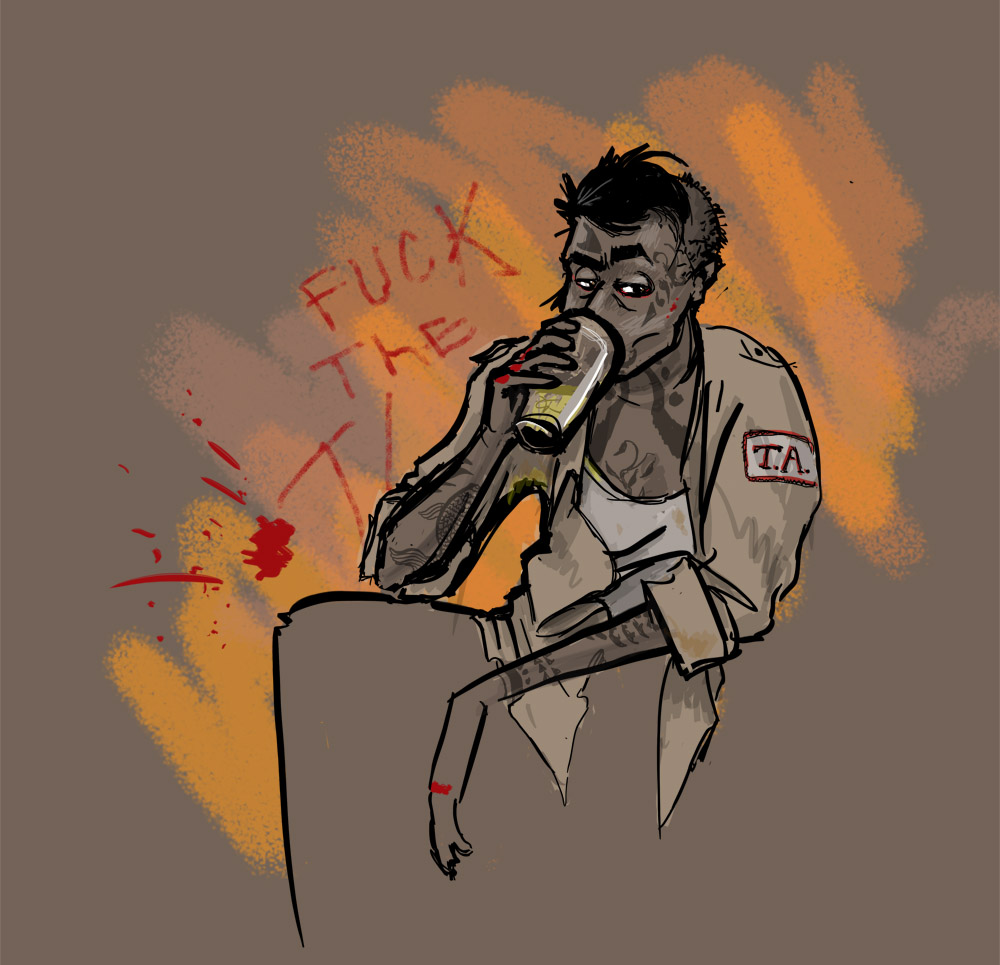
\includegraphics[width=12cm]{img/ch11_drunk_jaya.jpg}
\end{center}